\section{Hyperbolic Functions}\label{sec:hyperbolic}

\begin{goals}
\item What are hyperbolic functions?  
\item What properties do hyperbolic functions possess?
\end{goals} 

%---------------------------------------------
% SUBSECTION INTRODUCTION
%---------------------------------------------
\subsection*{Introduction}

The \textbf{hyperbolic functions} are a set of functions that have many applications to mathematics, physics, and engineering. Among many other applications, they are used to describe the formation of satellite rings around planets, to describe the shape of a rope hanging from two points, and have application to the theory of special relativity. This section defines the hyperbolic functions and describes many of their properties, especially their usefulness to calculus.


%-----------------------------------------------------------
% SUBSECTION HYPERBOLIC FUNCTIONS
%-----------------------------------------------------------
\subsection*{Hyperbolic Functions}

These functions are sometimes referred to as the ``hyperbolic trigonometric functions'' as there are many, many connections between them and the standard trigonometric functions. Figure~\ref{fig:6.8_hyperbolic} demonstrates one such connection. Just as cosine and sine are used to define points on the circle defined by $x^2+y^2=1$, the functions \textbf{hyperbolic cosine} and \textbf{hyperbolic sine} are used to define points on the hyperbola $x^2-y^2=1$.

\begin{marginfigure} % MARGIN FIGURE
\captionsetup[subfigure]{labelformat=empty}
\subfloat{\margingraphics{figures/fighf_circlearea}}

\subfloat{\margingraphics{figures/fighf_hyperbolaarea}}

\caption{Using trigonometric functions to define points on a circle and hyperbolic functions to define points on a hyperbola. The area of the shaded regions are included in them.}
\label{fig:6.8_hyperbolic}
\end{marginfigure}

\definition{Hyperbolic Functions\index{hyperbolic function!definition}}{%DEFINITION
\bmtwo
\begin{enumerate}[1)]
\item	 $\ds \sinh(x) = \frac{e^x-e^{-x}}2$
\item	 $\ds \cosh(x) = \frac{e^x+e^{-x}}2$
\item	 $\ds \tanh (x) = \frac{\sinh (x)}{\cosh (x)}$
\item	 $\ds \csch (x) = \frac{1}{\sinh (x)}$
\item	 $\ds \sech (x) = \frac{1}{\cosh (x)}$
\item	 $\ds \coth (x) = \frac{\cosh (x)}{\sinh (x)}$
\end{enumerate}
\emtwo
} % end definition

These hyperbolic functions are graphed in Figure~\ref{fig:6.8_hyperbolicgraphs}. In the graphs of $\cosh (x)$ and $\sinh (x)$, graphs of $e^x/2$ and $e^{-x}/2$ are included with dashed lines. As $x$ gets ``large,'' $\cosh (x)$ and $\sinh (x)$ each act like $e^x/2$; when $x$ is a large negative number, $\cosh (x)$ acts like $e^{-x}/2$ whereas $\sinh (x)$ acts like $-e^{-x}/2$.

\marginnote{\textbf{Pronunciation Note:} \par ``cosh'' rhymes with ``gosh,'' \par ``sinh'' rhymes with ``pinch,'' and \par ``tanh'' rhymes with ``ranch.''}

Notice the domains of $\tanh (x)$ and $\sech (x)$ are $(-\infty,\infty)$, whereas both $\coth (x)$ and $\csch (x)$ have vertical asymptotes at $x=0$. Also note the ranges of these function, especially $\tanh (x)$: as $x\to\infty$, both $\sinh (x)$ and $\cosh (x)$ approach $e^{-x}/2$, hence $\tanh (x)$ approaches $1$.

\begin{figure} %  FIGURE
\begin{center}
\begin{tabular}{cc}
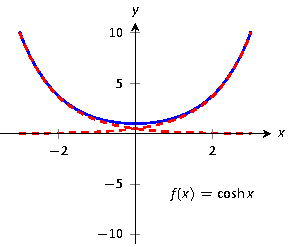
\includegraphics{figures/fighf_cosh}  & 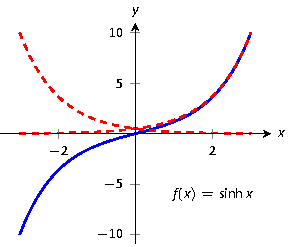
\includegraphics{figures/fighf_sinh} \\[20pt]
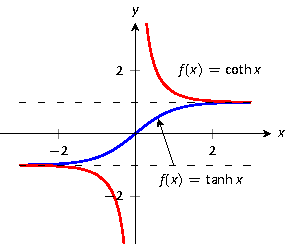
\includegraphics{figures/fighf_tanh_coth} &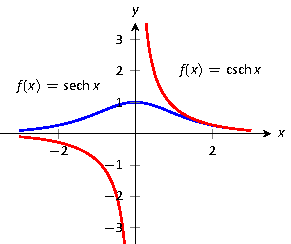
\includegraphics{figures/fighf_sech_csch}
\end{tabular}
\caption{Graphs of the hyperbolic functions.}
\label{fig:6.8_hyperbolicgraphs}
\end{center}
\end{figure}
 
The following example explores some of the properties of these functions that bear remarkable resemblance to the properties of their trigonometric counterparts.


\begin{example} \label{eg:6.8.1} % EXAMPLE
Use the definitions of the hyperbolic functions to rewrite the following expressions.
\bmtwo
\begin{enumerate}[1)]
\item	 $\cosh^2 (x)-\sinh^2(x)$
\item	 $\tanh^2 (x)+\sech^2 (x)$
\item	 $2\cosh (x)\sinh (x)$
\item	 $\frac{d}{dx}\big(\cosh (x)\big)$
\item	 $\frac{d}{dx}\big(\sinh (x)\big)$
\item	 $\frac{d}{dx}\big(\tanh (x)\big)$
\end{enumerate}
\emtwo

\solution
\begin{enumerate}[1)]
\item	 $\begin{aligned}[t]
 \cosh^2(x)-\sinh^2(x) &= \left(\frac{e^x+e^{-x}}2\right)^2 -\left(\frac{e^x-e^{-x}}2\right)^2\\
 						&= \frac{e^{2x}+2e^xe^{-x} + e^{-2x}}4 - \frac{e^{2x}-2e^xe^{-x} + e^{-2x}}4\\
 						&= \frac44=1.
\end{aligned}$\hfill

So $\cosh^2 (x)-\sinh^2(x)=1$.

\item	 $\begin{aligned}[t]
\tanh^2 (x)+\sech^2 (x) &=\frac{\sinh^2(x)}{\cosh^2 (x)} + \frac{1}{\cosh^2 (x)} \\
&= \frac{\sinh^2(x)+1}{\cosh^2 (x)}\qquad \text{\small Now use identity from \#1)}\\
&= \frac{\cosh^2 (x)}{\cosh^2 (x)} = 1
\end{aligned}$\hfill

So $\tanh^2 (x)+\sech^2 (x)=1$.

\item $\begin{aligned}[t]
2\cosh (x)\sinh (x) &= 2\left(\frac{e^x+e^{-x}}2\right)\left(\frac{e^x-e^{-x}}2\right) \\
&= 2 \cdot\frac{e^{2x} - e^{-2x}}4\\
&= \frac{e^{2x} - e^{-2x}}2 = \sinh (2x).\\
\end{aligned}$ \hfill
			
Thus $2\cosh (x)\sinh (x) = \sinh (2x)$.

\item  $\begin{aligned}[t]
\frac{d}{dx}\big(\cosh (x)\big) &= \frac{d}{dx}\left(\frac{e^x+e^{-x}}2\right) \\
&= \frac{e^x-e^{-x}}2\\
&= \sinh (x)
\end{aligned}\hfill$

So $\frac{d}{dx}\big(\cosh (x)\big) = \sinh (x).$
	
\item  $\begin{aligned}[t]
\frac{d}{dx}\big(\sinh (x)\big) &= \frac{d}{dx}\left(\frac{e^x-e^{-x}}2\right) \\
&= \frac{e^x+e^{-x}}2\\
&= \cosh (x)
\end{aligned}\hfill$

So $\frac{d}{dx}\big(\sinh (x)\big) = \cosh (x).$
	
\item  $\begin{aligned}[t]
\frac{d}{dx}\big(\tanh (x)\big) &= \frac{d}{dx}\left(\frac{\sinh (x)}{\cosh (x)}\right) \\
&= \frac{\cosh (x) \cosh (x) - \sinh (x) \sinh (x)}{\cosh^2 (x)}\\
&= \frac{1}{\cosh^2 (x)}\\
&= \sech^2 (x)
\end{aligned}\hfill$

So $\frac{d}{dx}\big(\tanh (x)\big) = \sech^2 (x).$	
\end{enumerate}

\end{example}%EXAMPLE

\begin{activity} \label{A:6.8.1} Compute the following limits.
\bmtwo
\begin{enumerate}[1)]
\item $\ds \lim_{x \rightarrow \infty} \cosh (x)$
\item $\ds \lim_{x \rightarrow \infty} \sinh (x) $
\item $\ds \lim_{x \rightarrow \infty} \tanh (x) $
\item $\ds \lim_{x \rightarrow \infty} (\cosh (x) - \sinh (x)) $
\end{enumerate}
\emtwo
\end{activity}
\begin{smallhint}
\ba
	\item Small hints for each of the prompts above.
\ea
\end{smallhint}
\begin{bighint}
\ba
	\item Big hints for each of the prompts above.
\ea
\end{bighint}
\begin{activitySolution}
\ba
	\item Solutions for each of the prompts above.
\ea
\end{activitySolution}
\aftera % ACTIVITY

The following concept summarizes many of the important identities relating to hyperbolic functions. Each can be verified by referring back to the definition of the hyperbolic functions.

\concept{Useful Hyperbolic Function Properties}{ %CONCEPT
\textbf{Basic Identities}\par
\bmtwo
\begin{enumerate}[1)]\small
\item $\cosh^2(x)-\sinh^2(x)=1$%
\index{hyperbolic function!identities}\index{hyperbolic function!derivatives}\index{hyperbolic function!integrals}\index{derivative!hyperbolic funct.}\index{integration!hyperbolic funct.}%
\item	$\tanh^2(x)+\sech^2(x)=1$
\item	$\coth^2(x)-\csch^2(x) = 1$
\item	$\cosh (2x)=\cosh^2(x)+\sinh^2(x)$
\item	$\sinh (2x) = 2\sinh (x)\cosh (x)$
\item	$\ds\cosh^2(x) = \frac{\cosh (2x)+1}{2}$
\item $\ds \sinh^2(x)=\frac{\cosh (2x)-1}{2}$
\end{enumerate}\normalsize
\emtwo
\textbf{Derivatives}
\bmtwo
\begin{enumerate}[1)]\small
\item $\frac{d}{dx}\big(\cosh (x)\big) = \sinh (x)$
\item $\frac{d}{dx}\big(\sinh (x)\big) = \cosh (x)$
\item $\frac{d}{dx}\big(\tanh (x)\big) = \sech^2 (x)$
\item $\frac{d}{dx}\big(\sech (x)\big) = -\sech (x)\tanh (x)$
\item $\frac{d}{dx}\big(\csch (x)\big) = -\csch (x)\coth (x)$
\item $\frac{d}{dx}\big(\coth (x)\big) = -\csch^2(x)$
\end{enumerate}\normalsize
\emtwo
\textbf{Integrals}
\bmtwo
\begin{enumerate}[1)]\small
\item $\ds\int \cosh (x)\ dx = \sinh (x)+C$
\item $\ds\int \sinh (x)\ dx = \cosh (x)+C$
\item $\ds\int \tanh (x)\ dx = \ln(\cosh (x)) +C$
\item $\ds\int \coth (x)\ dx = \ln|\sinh (x)\,|+C$
\end{enumerate}\normalsize
\emtwo
} %end CONCEPT

\begin{example} \label{eg:6.8.2} % EXAMPLE
Evaluate the following derivatives and integrals.

\begin{enumerate*}[1)]
\item	 $\ds\frac{d}{dx}\big(\cosh (2x)\big)$\hspace{.5cm}
\item	 $\ds\int \sech^2(7t-3)\ dt$\hspace{.5cm}
\item	 $\ds \int_0^{\ln (2)} \cosh (x)\ dx$
\end{enumerate*}

\solution
\begin{enumerate}[1)]
\item Using the Chain Rule directly, we have $\frac{d}{dx} \big(\cosh (2x)\big) = 2\sinh (2x)$.

Just to demonstrate that it works, let's also use the Basic Identity $\cosh (2x) = \cosh^2(x)+\sinh^2(x)$.
\begin{align*}
\frac{d}{dx}\big(\cosh (2x)\big) &= \frac{d}{dx}\big(\cosh^2(x)+\sinh^2(x)\big) \\
&= 2\cosh (x)\sinh (x)+ 2\sinh (x)\cosh (x)\\ 
&= 4\cosh (x)\sinh (x).
\end{align*}
Using another Basic Identity, we can see that $4\cosh (x)\sinh (x) = 2\sinh (2x)$. We get the same answer either way.

\item	  We employ substitution, with $u = 7t-3$ and $du = 7dt$. Then we have:
$$ \int \sech^2 (7t-3)\ dt = \frac17\tanh (7t-3) + C.$$

\item	 $\ds \int_0^{\ln (2)} \cosh (x)\ dx = \sinh (x)\Big|_0^{\ln (2)} = \sinh (\ln (2)) - \sinh (0) = \sinh(\ln (2)).$
\noindent We can simplify this last expression as $\sinh x$ is based on exponentials:
$$\sinh(\ln (2)) = \frac{e^{\ln (2)}-e^{-\ln (2)}}2 = \frac{2-1/2}{2} = \frac34.$$
\end{enumerate}

\end{example}%EXAMPLE

\begin{activity} \label{A:6.8.3} Evaluate the following integrals.
\bmtwo
\begin{enumerate}[1)]
\item $\ds \int \sinh(3x)+x^3 \ dx  $
\item $\ds \int \tanh(x) \ dx ) $
\item $\ds \int \cosh^2(x) \ dx  $
\item $\ds \int \frac{\sinh(x)}{1 +  \cosh^2(x)} \ dx $
\end{enumerate}
\emtwo
\end{activity}
\begin{smallhint}
\ba
	\item Small hints for each of the prompts above.
\ea
\end{smallhint}
\begin{bighint}
\ba
	\item Big hints for each of the prompts above.
\ea
\end{bighint}
\begin{activitySolution}
\ba
	\item Solutions for each of the prompts above.
\ea
\end{activitySolution}
\aftera % ACTIVITY

%-----------------------------------------------------------
% SUBSECTION INVERSE HYPERBOLIC FUNCTIONS
%-----------------------------------------------------------
\subsection*{Inverse Hyperbolic Functions}

Just as the inverse trigonometric functions are useful in certain integrations, the inverse hyperbolic functions are useful with others. Table~\ref{T:hfinverse2} shows the restrictions on the domains to make each function one-to-one and the resulting domains and ranges of their inverse functions. Their graphs are shown in Figure~\ref{fig:hfinverse1}.\index{hyperbolic function!inverse}

\begin{margintable}[0cm] % MARGIN TABLE
\begin{tabular}{ccc}
Function & Domain & Range\\ \hline
$\cosh (x)$ & $[0,\infty)$ & $[1,\infty)$\\
$\sinh (x)$ & $(-\infty,\infty)$ & $(-\infty,\infty)$\\
$\tanh (x)$ & $(-\infty,\infty)$ & $(-1,1)$\\
$\sech (x)$ & $[0,\infty)$ & $(0,1]$ \\
$\csch (x)$ & $(-\infty,0) \cup (0,\infty)$ & $(-\infty,0) \cup (0,\infty)$\\
$\coth (x)$ & $(-\infty,0) \cup (0,\infty)$ & $(-\infty,-1) \cup (1,\infty)$
\end{tabular}
\caption{Domains and ranges of the hyperbolic functions.} \label{T:6.8_hyper1}
\end{margintable}

\begin{margintable}[0cm] % MARGIN TABLE
\begin{tabular}{ccc}
Function & Domain & Range\\ \hline
\rule{0pt}{10pt}$\cosh^{-1} (x)$ & $[1,\infty)$ & $[0,\infty)$ \\
$\sinh^{-1} (x)$ & $[-\infty,\infty)$ & $[-\infty,\infty)$\\
$\tanh^{-1} (x)$ & $(-1,1)$ & $(-\infty,\infty)$\\
$\sech^{-1} (x)$ & $(0,1]$ & $[0,\infty)$ \\
$\csch^{-1} (x)$ & $(-\infty,0) \cup (0,\infty)$ & $(-\infty,0) \cup (0,\infty)$\\
$\coth^{-1} (x)$ & $(-\infty,-1) \cup (1,\infty)$ & $(-\infty,0) \cup (0,\infty)$
\end{tabular}
\caption{Domains and ranges of the inverse hyperbolic functions.}\label{T:hfinverse2}
\end{margintable}

Because the hyperbolic functions are defined in terms of exponential functions, their inverses can be expressed in terms of logarithms. It is often more convenient to refer to $\sinh^{-1} x$ than to $\ln\big(x+\sqrt{x^2+1}\big)$, especially when one is working on theory and does not need to compute actual values. On the other hand, when computations are needed, technology is often helpful but many hand-held calculators lack a \textit{convenient} $\sinh^{-1}x$ button. (Often it can be accessed under a menu system, but not conveniently.) In such a situation, the logarithmic representation is useful.

In next concept, both the inverse hyperbolic and logarithmic function representations of the antiderivative are given. Again, these latter functions are often more useful than the former. Note how inverse hyperbolic functions can be used to solve integrals we used Trigonometric Substitution to solve in Section~\ref{S:5.3.TrigSub}.

\begin{figure} % FIGURE
\begin{minipage}{1.3\textwidth}
\begin{tabular}{ccc}
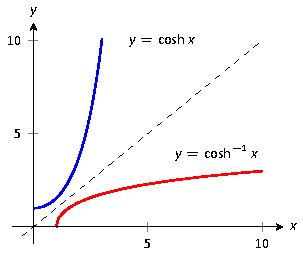
\includegraphics[scale=0.95]{figures/fighfarccosh} & \ \hskip 15pt\ &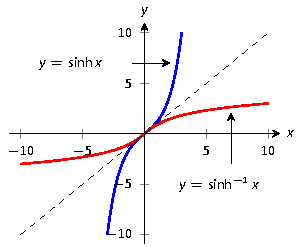
\includegraphics[scale=0.95]{figures/fighfarcsinh}\\[15pt]
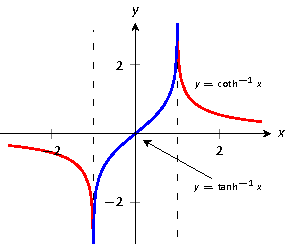
\includegraphics[scale=0.95]{figures/fighfarctanharccoth} & &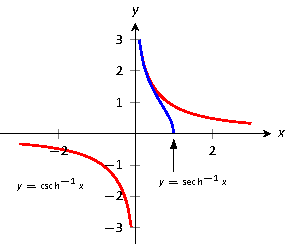
\includegraphics[scale=0.95]{figures/fighfarcsecharccsch}
\end{tabular}
\captionsetup{type=figure}%
\caption{Graphs of the hyperbolic functions and their inverses.}\label{fig:hfinverse1}
\end{minipage}
\end{figure}

\concept{Logarithmic definitions of Inverse Hyperbolic Functions}{ % CONCEPT 
\begin{enumerate}[1)]
\item $\ds\cosh^{-1}(x)=\ln\big(x+\sqrt{x^2-1}\big);\ x\geq1$\index{hyperbolic function!inverse!logarithmic def.}\rule[-10pt]{0pt}{20pt}
\item $\ds\tanh^{-1}(x) = \frac12\ln\left(\frac{1+x}{1-x}\right);\ |x|<1$\rule[-10pt]{0pt}{20pt}
\item $\ds \sech^{-1}(x) = \ln\left(\frac{1+\sqrt{1-x^2}}x\right);\ 0<x\leq1$\rule[-10pt]{0pt}{20pt}
\item $\ds\sinh^{-1}(x) = \ln\big(x+\sqrt{x^2+1}\big)$\rule[-10pt]{0pt}{20pt}
\item	 $\ds\coth^{-1}(x) = \frac12\ln\left(\frac{x+1}{x-1}\right);\ |x|>1$\rule[-10pt]{0pt}{20pt}
\item $\ds\csch^{-1}(x) = \ln\left(\frac1x+\frac{\sqrt{1+x^2}}{|x|}\right);\ x\neq0$\rule[-10pt]{0pt}{20pt}
\end{enumerate}
} % END CONCEPT

The following concepts give the derivatives and integrals relating to the inverse hyperbolic functions. 

\concept{Derivatives Involving Inverse Hyperbolic Functions \index{derivative!inverse hyper.}\index{hyperbolic function!inverse!derivative}}{% CONCEPT
\begin{enumerate}[1)]
\item $\ds\frac{d}{dx}\big(\cosh^{-1} (x)\big) = \frac{1}{\sqrt{x^2-1}};\ x>1$
\item $\ds\frac{d}{dx}\big(\sinh^{-1} (x)\big) = \frac{1}{\sqrt{x^2+1}}$
\item $\ds\frac{d}{dx}\big(\tanh^{-1} (x)\big) = \frac{1}{1-x^2};\ |x|<1$
\item $\ds\frac{d}{dx}\big(\sech^{-1} (x)\big) = \frac{-1}{x\sqrt{1-x^2}}; 0<x<1$
\item $\ds\frac{d}{dx}\big(\csch^{-1} (x)\big) = \frac{-1}{|x|\sqrt{1+x^2}};\ x\neq0$
\item $\ds\frac{d}{dx}\big(\coth^{-1} (x)\big) = \frac{1}{1-x^2};\ |x|>1$
\end{enumerate}
}% end concept

\begin{activity} \label{A:6.8.2} Differentiate the following functions.
\begin{enumerate}[1)]
\item $\ds \frac{d}{dx}( \sinh(3x+x^3) )  $
\item $\ds \frac{d}{dx}( \arccos( \tanh(x) ) ) $
\item $\ds \frac{d}{dx}( \sinh^{-1} (3 \tanh (3x)) ) $
\item $\ds \frac{d}{dx}( \cosh^{-1}(\sqrt{x^2+1})  ) $
\item Show that $f(t) = \cosh(\sqrt{3}t) - \frac{2}{\sqrt{3}}\sinh(\sqrt{3}t)$ is a solution to the differential equation $f''-3f=0$.  
\end{enumerate}
\end{activity}
\begin{smallhint}
\ba
	\item Small hints for each of the prompts above.
\ea
\end{smallhint}
\begin{bighint}
\ba
	\item Big hints for each of the prompts above.
\ea
\end{bighint}
\begin{activitySolution}
\ba
	\item Solutions for each of the prompts above.
\ea
\end{activitySolution}
\aftera % ACTIVITY

\concept{Integrals Involving Inverse Hyperbolic Functions \index{integration!inverse hyper.}\index{hyperbolic function!inverse!integration}}{% CONCEPT
\begin{enumerate}[1)]
\item \begin{align*}
\ds\int \frac{1}{\sqrt{x^2-a^2}}\ dx &= \cosh^{-1}\left(\frac xa\right)+C;\ 0<a<x\\
&= \ds\ln\Big|x+\sqrt{x^2-a^2}\Big|+C
\end{align*}

\item \begin{align*}
\ds\int \frac{1}{\sqrt{x^2+a^2}}\ dx &= \sinh^{-1}\left(\frac xa\right)+C;\ a>0 \\
&= \ds\ln\Big|x+\sqrt{x^2+a^2}\Big|+C
\end{align*}

\item \begin{align*}
\ds\int \frac{1}{a^2-x^2}\ dx &= \left\{\begin{array}{ccc} \frac1a\tanh^{-1}\left(\frac xa\right)+C & & x^2<a^2 \\ \\
\frac1a\coth^{-1}\left(\frac xa\right)+C & & a^2<x^2 \end{array}\right.\\
&= \ds\frac12\ln\left|\frac{a+x}{a-x}\right|+C
\end{align*}

\item \begin{align*}
\ds\int \frac{1}{x\sqrt{a^2-x^2}}\ dx &= -\frac1a\sech^{-1}\left(\frac xa\right)+C;\ 0<x<a \\
&= \ds \frac1a \ln\left(\frac{x}{a+\sqrt{a^2-x^2}}\right)+C 
\end{align*}

\item	 \begin{align*}
\ds\int \frac{1}{x\sqrt{x^2+a^2}}\ dx &= -\frac1a\csch^{-1}\left|\frac xa\right| + C;\ x\neq 0,\ a>0 \\
&= \ds \frac1a \ln\left|\frac{x}{a+\sqrt{a^2+x^2}}\right|+C 
\end{align*}
\end{enumerate}
}% end CONCEPT

\begin{example} \label{eg:6.8.3} % EXAMPLE
Evaluate the following.

\begin{enumerate*}[1)]
\item	$\ds \frac{d}{dx}\left[\cosh^{-1}\left(\frac{3x-2}{5}\right)\right]$ \hspace{.25cm}
\item	$\ds \int\frac{1}{x^2-1}\ dx$ \hspace{.25cm}
\item	$\ds \int \frac{1}{\sqrt{9x^2+10}}\ dx$
\end{enumerate*}

\solution
\begin{enumerate}[1)]
\item	 Applying the concepts along with the Chain Rule gives:
$$\frac{d}{dx}\left[\cosh^{-1}\left(\frac{3x-2}5\right)\right] = \frac{1}{\sqrt{\left(\frac{3x-2}5\right)-1}}\cdot\frac35.$$

\item Multiplying the numerator and denominator by $(-1)$ gives: $\ds \int \frac{1}{x^2-1}\ dx = \int \frac{-1}{1-x^2}\ dx$. The second integral can be solved with a direct application of item \#3 from the integral concepts, with $a=1$. Thus
\begin{align*}
\int \frac{1}{x^2-1}\ dx &= -\int \frac{1}{1-x^2}\ dx  \\
&= \left\{\begin{array}{ccc} -\tanh^{-1}\left(x\right)+C & & x^2<1 \\ \\ -\coth^{-1}\left(x\right)+C & & 1<x^2 \end{array}\right. \\
&=-\frac12\ln\left|\frac{x+1}{x-1}\right|+C\\
&=\frac12\ln\left|\frac{x-1}{x+1}\right|+C.
\end{align*}

%The key to linking the two seemingly different answers together is Figure \ref{fig:hfinverse5}, where the logarithmic definitions of the inverse hyperbolic functions are given. Note that the definitions of $\tanh^{-1}x$ and $\coth^{-1}x$ are very similar; the conditions placed on $|x|$ ensure that the argument of $\ln$ is always positive. Thus one could say 
%$$\frac12\ln\left|\frac{x+1}{x-1}\right| = \left\{\begin{array}{ccc} \tanh^{-1}x+C & & |x|<1 \\ \\
%\coth^{-1}x+C & & |x|>1 \end{array}\right..$$
%
%We reconcile the two answers by returning to Equation \ref{eq:hf3} and continuing:
%\begin{align*}
%\int \frac{1}{x^2-1}\ dx &= \int \frac{-1}{1-x^2}\ dx \\
%			&= \left\{\begin{array}{ccc} -\frac1a\tanh^{-1}\left(\frac xa\right)+C & & x^2<a^2 \\ \\
%-\frac1a\coth^{-1}\left(\frac xa\right)+C & & a^2<x^2 \end{array}\right. \\
%			&= -\frac12\ln\left|\frac{x+1}{x-1}\right|+C \\
%			&= -\frac12\ln|x+1| + \frac12\ln|x-1| +C,
%\end{align*}
%matching the answer previously obtained.

\item	 This requires a substitution; let $u = 3x$, hence $du = 3dx$. We have 
\begin{align*}
\int \frac{1}{\sqrt{9x^2+10}}\ dx &= \frac13\int\frac{1}{\sqrt{u^2+10}}\ du. \\
\intertext{Note $a^2=10$, hence $a = \sqrt{10}.$ Now apply the integral rule.}
 &= \frac13 \sinh^{-1}\left(\frac{3x}{\sqrt{10}}\right) + C \\
 &= \frac13 \ln \Big|3x+\sqrt{9x^2+10}\Big|+C.
\end{align*}
\end{enumerate}

\end{example}%EXAMPLE

%-----------------------------------------------------------
% SUMMARY
%-----------------------------------------------------------
\begin{summary}
\item The hyperbolic functions are similar to trigonometric functions in that they both can represent distances from the origin to a conic section.
\end{summary}

\clearpage

%--------------
% EXERCISES
%--------------
\begin{adjustwidth*}{}{-2.25in}
\textbf{{\large Exercises}}
\setlength{\columnsep}{25pt}
\begin{multicols*}{2}

\noindent {\normalsize Problems} \small

\noindent{\bf In Exercises 1--8, verify the identity.}

\begin{enumerate}[1)]
\item $\coth^2 x-\csch^2x=1$

\item $\cosh 2x = \cosh^2x+\sinh^2x$

\item $\ds\cosh^2x = \frac{\cosh2x+1}{2}$

\item $\ds\sinh^2x = \frac{\cosh2x-1}{2}$

\item $\ds\frac{d}{dx}\left[\sech x\right] = -\sech x\tanh x$

\item $\ds\frac{d}{dx}\left[\coth x\right] = -\csch^2x$

\item $\ds \int \tanh x\ dx  = \ln (\cosh x) + C$

\item $\ds \int \coth x\ dx  = \ln |\sinh x| + C$
\end{enumerate}

\noindent{\bf In Exercises 9--19, differentiate the given function.}

\begin{enumerate}[1),resume]

\item $f(x) = \cosh 2x$

\item $f(x) = \tanh (x^2)$

\item $f(x) = \ln(\sinh x)$

\item $f(x) = \sinh x\cosh x$

\item $f(x) = x\sinh x-\cosh x$

\item $f(x) = \sech^{-1} (x^2)$

\item $f(x) = \tanh^{-1} (\cos x)$

\item $f(x) = \cosh^{-1} (\sec x)$

\item $f(x) = \sinh^{-1} (3x)$

\item $f(x) = \cosh^{-1} (2x^2)$

\item $f(x) = \tanh^{-1} (x+5)$
\end{enumerate}

\noindent{\bf In Exercises 20--24, produce the equation of the line tangent to the function at the given $x$-value.}

\begin{enumerate}[1),resume]
\item $f(x) = \sinh x$ at $x=0$
\item $f(x) = \cosh x$ at $x=\ln 2$
\item $f(x) = \sech^2 x$ at $x=\ln 3$
\item $f(x) = \sinh^{-1} x$ at $x=0$
\item $f(x) = \cosh^{-1} x$ at $x=\sqrt 2$
\end{enumerate}

\noindent{\bf In Exercises 25--36, evaluate the given indefinite integral.}

\begin{enumerate}[1),resume]
\item $\ds \int \tanh (2x)\ dx$
\item $\ds \int \cosh (3x-7)\ dx$
\item $\ds \int \sinh x\cosh x\ dx$
\item $\ds \int \frac{1}{9-x^2}\ dx$
\item $\ds \int \frac{2x}{\sqrt{x^4-4}}\ dx$
\item $\ds \int \frac{\sqrt{x}}{\sqrt{1+x^3}}\ dx$
\item $\ds \int \frac{1}{x^4-16}\ dx$
\item $\ds \int \frac{1}{x^2+x}\ dx$
\item $\ds \int \frac{e^x}{e^{2x}+1}\ dx$
\item $\ds \int \sinh^{-1}x \ dx$
\item $\ds \int \tanh^{-1}x \ dx$
\item $\ds \int \sech x \ dx$ \quad(Hint: mutiply by $\frac{\cosh x}{\cosh x}$; set $u = \sinh x$.)

\end{enumerate}

\noindent{\bf In Exercises 37--39, evaluate the given definite integral.}

\begin{enumerate}[1),resume]
\item $\ds \int_{-1}^1 \sinh x \ dx$
\item $\ds \int_{-\ln 2}^{\ln 2} \cosh x \ dx$
\item $\ds \int_{0}^{1} \tanh^{-1} x \ dx$
\end{enumerate}

%------------------------------------------
% END OF EXERCISES ON FIRST PAGE
%------------------------------------------
\end{multicols*}
\end{adjustwidth*}

\afterexercises 

\cleardoublepage